% ======================================================================================================
% NOTES, TODOS
% ======================================================================================================
\subsection{Search Result and Bibliometric Analysis}

After completion of the selection process, which involved applying inclusion and exclusion criteria and eliminating duplicate studies, a total of 73 research papers were considered eligible for further review and analysis. The accompanying pie chart (see Figure \ref{fig:archive-itemtype}) reveals that IEEE was the primary publisher of the selected papers, accounting for 49 of them. SpringerLink was the second largest contributor, with 14 publications, while Elsevier (4), ACM (3), MDPI (1), Pergamon (1) and SpieDigitalLibrary (1) each account for the lowest contribution of publications. The second right side of the pie chart also demonstrates that the majority of the selected papers were sourced from Web of Science and Scopus, followed by IEEE and SpringerLink. The distribution of publication types among the 74 selected papers is worth nothing. Of these papers, 60\% (i.e., 44 papers) were published as conference papers, whereas the remaining 40\% (i.e., 29 papers) were in the form of journal articles.



% \begin{figure}
% \includesvg[width=0.5\textwidth]{images/svg/databases.svg}
% \includesvg[width=0.5\textwidth]{images/svg/itemtype.svg}
% \svgcaption{This is the label for the SVG image.}
% \label{fig:image}
% \end{figure}

\begin{figure}[H]    
    \caption{An Analysis of Paper Distribution Based on Source and Publisher.}
    \centring
    \begin{subfigure}[b]{0.45\textwidth}
    \caption{Number of selected papers per publisher.}
        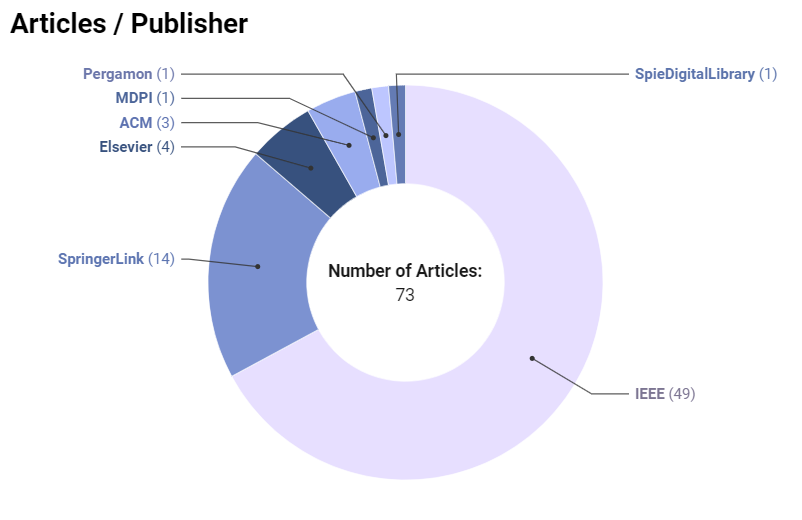
\includegraphics[width=\textwidth]{images/articles_per_publisher_2.png}
        % \includesvg[width=\textwidth]{images/svg/databases.svg}
    \end{subfigure}
    \begin{subfigure}[b]{0.45\textwidth}
    \caption{Number of selected papers per source.}
        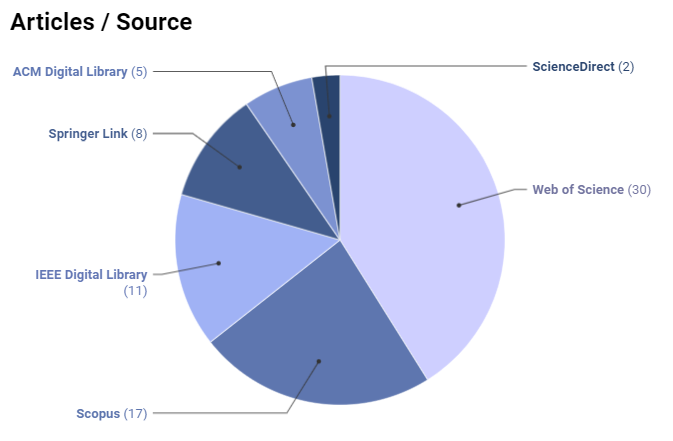
\includegraphics[width=\textwidth]{images/articles_per_source_pie.png}
        % \includesvg[width=\textwidth]{images/svg/itemtype.svg}
    \end{subfigure}
    \label{fig:archive-itemtype}
\end{figure}
 
Analysis of the distribution of selected papers based on publication year revealed that the majority of articles were published in 2022 and 2021. Furthermore, the bar chart illustrates a general upward trend in the number of publications addressing security concerns for industries utilising Digital Twin and (I)IoT applications. This trend indicates that there is a growing interest and concern among researchers in the field of Digital Twin and (I)IoT security, and highlights the relevance of this systematic literature review.

\begin{figure}[H]    
    \caption{Yearly Publication Statistics: Investigating the Number of Papers Published}
    % \includesvg[width=0.9\textwidth]{images/svg/pub_year_white_bg.svg}
    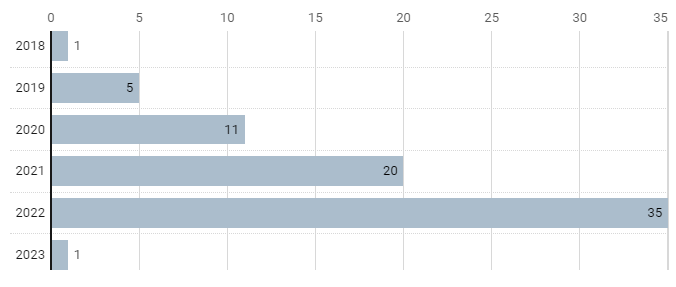
\includegraphics[width=\textwidth]{images/year8.png}
    \label{fig:bar-chart-yaer}
\end{figure}

To gain a deeper understanding of the trending topics within the 73 selected papers published between 2017 and 2023, a frequency analysis of keywords was conducted. This analysis was performed by extracting keywords that appeared more than three times in the abstracts and keyword sections of the articles, using the VOSviewer tool. Further filtering and sensitization was applied to create a shortlist of keywords. Additionally, keywords which have similar meanings with different spellings and variations were merged. The resulting frequency analysis of keywords, illustrated in Figure \ref{fig:alluvial-key}, provides valuable insight into the key themes and concepts that are prevalent in current research on the topic of Digital Twin and IoT security. This analysis can help guide future research by identifying areas where there is a need for further investigation and providing a sense of the current state of the field.


\begin{figure}[H]
    % \includesvg[width=0.9\textwidth]{images/svg/key_buble.svg}
    % 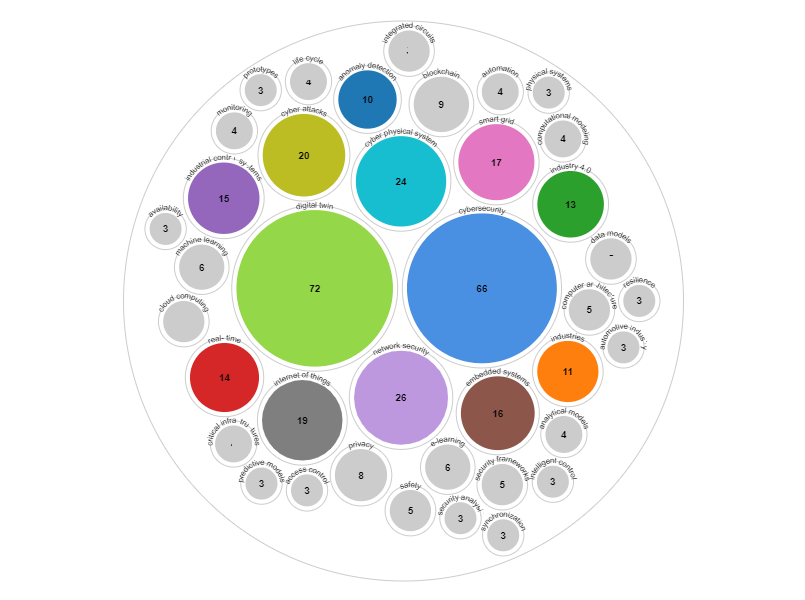
\includegraphics[width=\textwidth]{images/svg/key_buble.png}
    \caption{Frequency of keywords from abstract and keywords of 73 papers}
    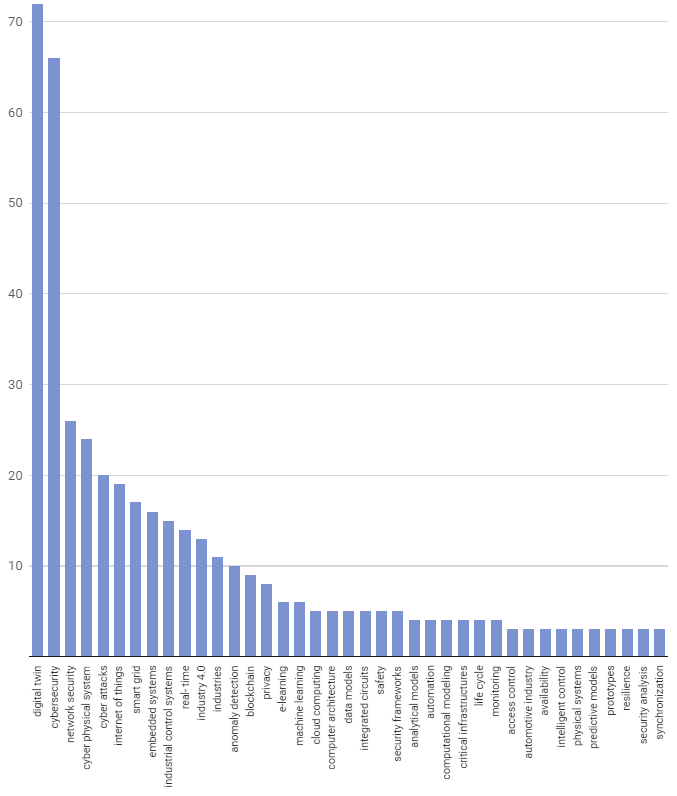
\includegraphics[width=0.8\textwidth]{images/keyword_occurance.png}
    \label{fig:alluvial-key}
\end{figure}
In this study, 73 papers were analyzed to generate a list of 1187 keywords using VOSViewer. During our analysis, we utilized a thesaurus text file to merge keywords with similar semantic meanings.

For instance, we replaced artificial intelligence and deep learning with machine learning, and intrusion detection with anomaly detection. We also merged related terms such as cyber-attacks, denial-of-service attacks, cyber attacks, and computer crime into a single term - cyber attacks. Similarly, we combined control systems under the term industrial control system and grouped electric power transmission network and smart power grids as smart grid. We further streamlined our findings by using industry 4.0 as an umbrella term for smart manufacturing and replaced real-time system with real-time.

Moreover, we limited the results to the top 87 keywords that appeared at least 3 times within the original list of 1187 keywords.  


The analysis of the selected papers using VOSviewer software revealed that which terms were frequently mentioned in the abstract and keyword section of the paper. The most frequently mentioned terms were "digital twin" with 72 occurrences, followed by "cybersecurity" with 66 occurrences, "cyberphysical system" with 24 occurrences, "cyber attacks" with 20 occurrences, "internet of things" with 19 occurrences, and "embedded systems" with 17 occurrences. This analysis highlights the key themes and concepts that are prevalent in current research on the topic of Digital Twin and IoT security. The high frequency of the term "digital twin" indicates the centrality of this concept in the field and the importance of understanding its role in ensuring the security of industries utilizing DT and IoT applications. The frequent mention of terms such as "cybersecurity" and "cyber attacks" further emphasizes the need for robust security measures to protect these systems from malicious actors.Additionally, the presence of terms such as "cyberphysical system" and "embedded systems" highlights the need for interdisciplinary research and collaboration between experts in fields such as computer science, engineering, and physics to effectively address the security challenges facing Digital Twin and IoT.

In order to gain further insights into the evolution of research in the field of Digital Twin and IoT security, a keyword co-relationship network analysis was extracted from VOSviewer tool. This analysis aimed to identify clusters of related items and visualise the relationships between keywords over time. The results of this analysis revealed that in the early days of research on Digital Twin, keywords such as "monitoring", "safety", "prototypes", "resilience", "software", and "tools" were frequently mentioned, which suggests that the primary focus of research at that time was on utilising Digital Twin as a visual aiding tool. However, more recent research is characterized by the frequent mention of emerging technologies such as "blockchain," "machine learning," "e-learning" "5G," and "privacy" This indicates that the development of Digital Twin has shifted towards utilising these technologies and augment Digital Twin to provide more service other than used as a model.



\begin{figure}[H]
    % \centering    
    \caption{keyword co-relationship from VOSviewer}
    % 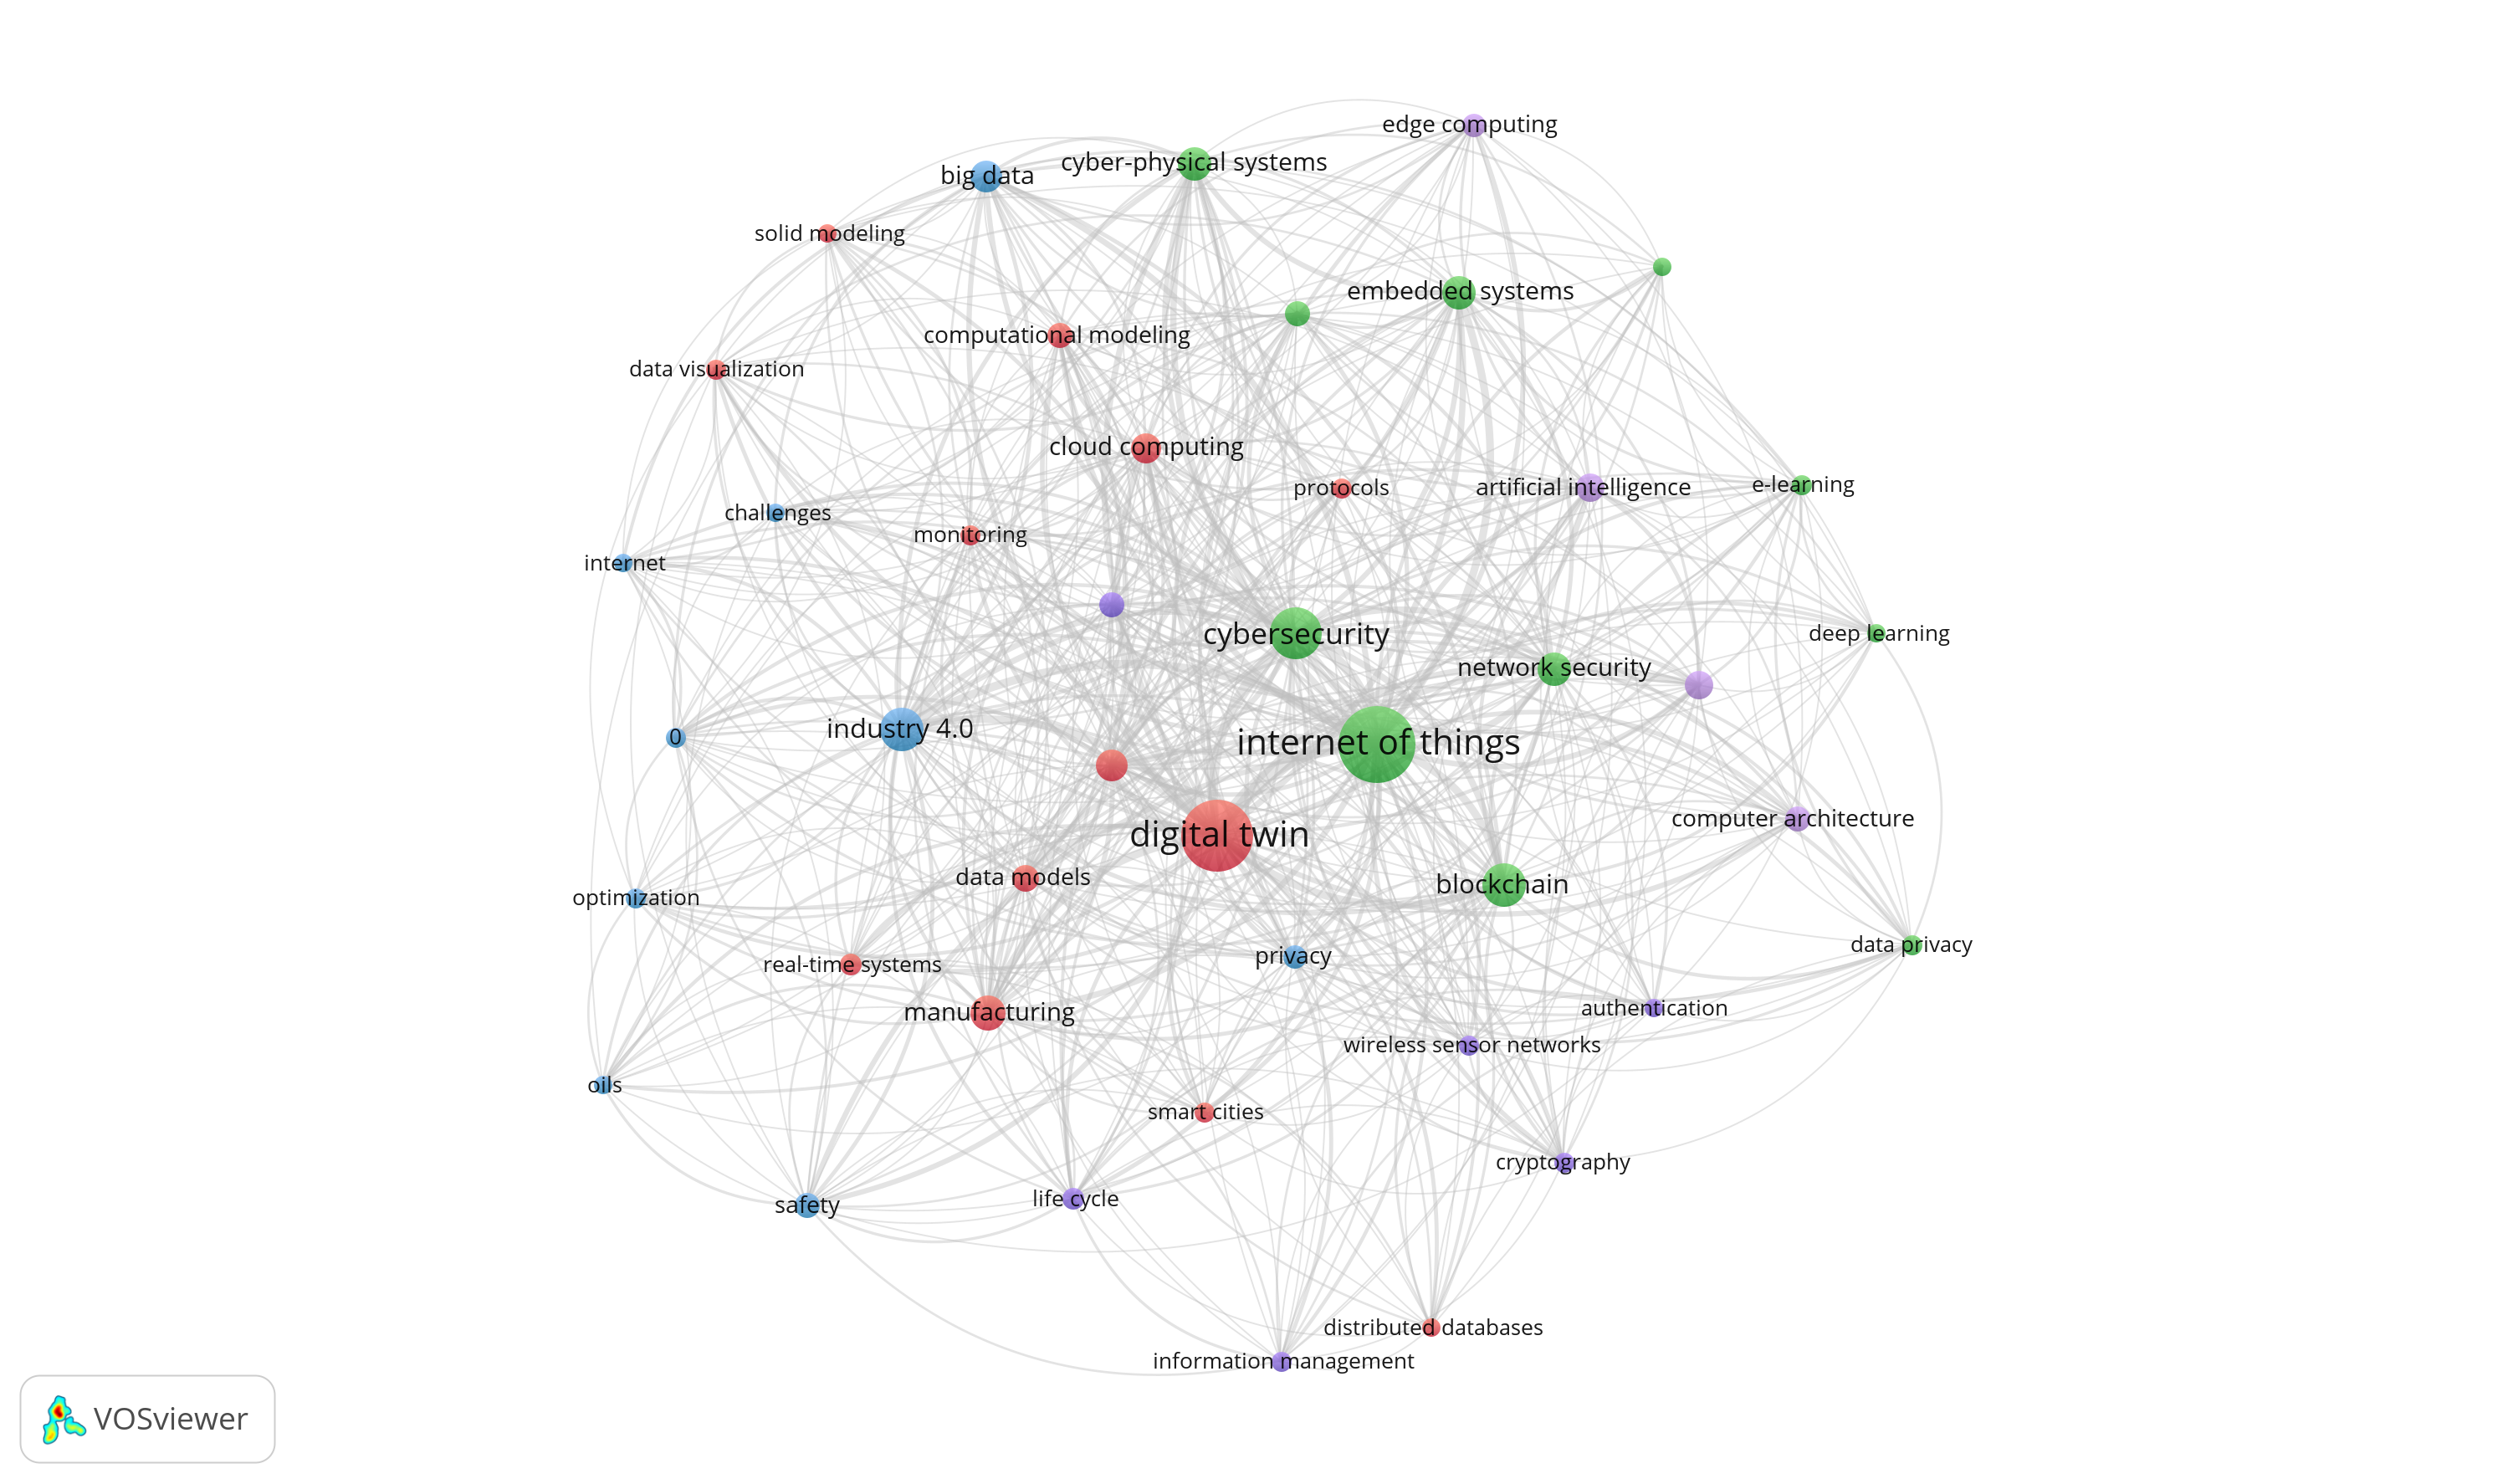
\includegraphics[width=1.5\textwidth, center]{images/vos_key_cooc_6_final.png}
    \includesvg[width=\textwidth]{images/svg/vos_co_time_2.svg}
    % \includesvg[inkscapelatex=false,width=0.95\columnwidth]{images/key_belt.svg}
    \label{fig:co-occurrence-vosv}
\end{figure}

The analysis of the co-occurrence of keywords in the selected articles, as represented in Figure \ref{fig:co-occurrence-vosv}, reveals the identification of five clusters. These clusters, as defined by the VOSviewer documentation, are groups of terms that exhibit a high degree of relatedness. Cluster one encompasses terms related to 5G technology, machine learning, real-time security analysis, security frameworks, access control, and automation. Cluster two comprises of keywords such as cybersecurity, data models, digital twin, internet of things, privacy, prototypes, safety, and cloud computing. The third cluster encompasses terms such as those related to the automotive industry, availability, blockchain, industry 4.0, industrial control systems, system life cycles, intelligent control, software, and tools. The fourth cluster is comprised of analytical models, anomaly detection, cyber-attacks, monitoring, resilience, critical infrastructure, integrated circuits, and physical systems. The final cluster includes terms such as cyber-physical systems, e-learning, embedded systems, predictive models, and smart grids.